\chapter{Binary Search}\label{ch:binary_search}
Just to memorize the template code below and everything will be fine.

\begin{lstlisting}
int BinarySearch(std::vector<int>& nums, int target) {
  int left = 0;
  int right = nums.size() - 1;
  while (left <= right) {
    int mid = left + (right - left) / 2;
    if (target == nums[mid]) {
      return mid;
    } else if (target < nums[mid]) {
      right = mid - 1;
    } else {
      left = mid + 1;
    }
  }
  return -1;
}
\end{lstlisting}

Binary search keeps narrowing down the search range by half, looking for the target until it's found or the range is invalid.
\begin{itemize}
\item {\colorbox{CodeBackground}{\lstinline|mid = left + (right - left) / 2|}}, check if {\colorbox{CodeBackground}{\lstinline|nums[mid]|}} is equal to {\colorbox{CodeBackground}{\lstinline|target|}}.
\item When {\colorbox{CodeBackground}{\lstinline|target|}} is to the left of {\colorbox{CodeBackground}{\lstinline|mid|}}, the search range is adjusted by {\colorbox{CodeBackground}{\lstinline|right = mid - 1|}}.
\item Similarly, when {\colorbox{CodeBackground}{\lstinline|target|}} is to the right of {\colorbox{CodeBackground}{\lstinline|mid|}},  the search range is adjusted by {\colorbox{CodeBackground}{\lstinline|left = mid + 1|}}.
\end{itemize}\mbox{}

At a special step where {\colorbox{CodeBackground}{\lstinline|right == left + 1|}} ($\Rightarrow$ {\colorbox{CodeBackground}{\lstinline|mid = left|}}), there are several scenarios:
\begin{enumerate}
\item If {\colorbox{CodeBackground}{\lstinline|target == nums[left]|}}, in the next iteration: {\colorbox{CodeBackground}{\lstinline|left|}} is fixed, {\colorbox{CodeBackground}{\lstinline|right = right - 1|}}, and the correct index is returned.
\item Similarly, if {\colorbox{CodeBackground}{\lstinline|target = nums[right]|}}, in the next iteration: {\colorbox{CodeBackground}{\lstinline|right|}} is fixed, {\colorbox{CodeBackground}{\lstinline|left = left + 1|}}, and the correct index is returned.
\item If {\colorbox{CodeBackground}{\lstinline|nums[left] < target < nums[right]|}}, {\colorbox{CodeBackground}{\lstinline|left = left + 1|}}, and then {\colorbox{CodeBackground}{\lstinline|target < nums[left]|}} $\Rightarrow$ Jump to case $4$.
\item If {\colorbox{CodeBackground}{\lstinline|target < nums[left]|}}, {\colorbox{CodeBackground}{\lstinline|left|}} is fixed and {\colorbox{CodeBackground}{\lstinline|right|}} will finally go beyond {\colorbox{CodeBackground}{\lstinline|left|}}, breaking the loop.
\item Similarly, if {\colorbox{CodeBackground}{\lstinline|target > nums[right]|}}, {\colorbox{CodeBackground}{\lstinline|right|}} is fixed and {\colorbox{CodeBackground}{\lstinline|left|}} will finally go beyond {\colorbox{CodeBackground}{\lstinline|right|}}, breaking the loop.
\end{enumerate}

\section{LC 0035 - Search Insert Position in Sorted Array}
Given a \ul{non-empty} \ul{sorted} integer array {\colorbox{CodeBackground}{\lstinline|nums|}} of \ul{distinct values} and a {\colorbox{CodeBackground}{\lstinline|target|}}, return:
\begin{itemize}
	\item the index of {\colorbox{CodeBackground}{\lstinline|target|}}, if the {\colorbox{CodeBackground}{\lstinline|target|}} is in {\colorbox{CodeBackground}{\lstinline|nums|}};
	\item the index where {\colorbox{CodeBackground}{\lstinline|target|}} would be if it were inserted in order, if the {\colorbox{CodeBackground}{\lstinline|target|}} is not in {\colorbox{CodeBackground}{\lstinline|nums|}};
\end{itemize}

Example:
\begin{itemize}
	\item {\colorbox{CodeBackground}{\lstinline|nums = [1,3,5,6], target = 5 --> 2|}}
	\item {\colorbox{CodeBackground}{\lstinline|nums = [1,3,5,6], target = 2 --> 1|}}
	\item {\colorbox{CodeBackground}{\lstinline|nums = [1,3,5,6], target = 7 --> 4|}}
\end{itemize}

\subsection*{Solution - Binary Search}
\begin{lstlisting}
int searchInsert(std::vector<int>& nums, int target) {
	int left = 0;
	int right = nums.size() - 1;
	while (left <= right) {
		int mid = left + (right - left) / 2;
		if (nums[mid] == target) {
			return mid;
		} else if (nums[mid] < target) {
			left = mid + 1;
		} else {
			right = mid - 1;
		}
	}
	return left;
}
\end{lstlisting}

\section{LC 0074 - Search in Sorted 2D Matrix}
You are given a \ul{non-empty} {\colorbox{CodeBackground}{\lstinline|m x n|}} integer matrix {\colorbox{CodeBackground}{\lstinline|matrix|}} with the following two properties:
\begin{itemize}
	\item Each \ul{row} is sorted in \ul{non-decreasing order}.
	\item The first integer of each row is greater than the last integer of the previous row.
\end{itemize}

Given an integer {\colorbox{CodeBackground}{\lstinline|target|}}, return {\colorbox{CodeBackground}{\lstinline|true|}} if {\colorbox{CodeBackground}{\lstinline|target|}} is in {\colorbox{CodeBackground}{\lstinline|matrix|}} or {\colorbox{CodeBackground}{\lstinline|false|}} otherwise. \\

Examples:
\begin{itemize}
	\item {\colorbox{CodeBackground}{\lstinline|matrix = [[1,3,5,7],[10,11,16,20],[23,30,34,60]], target = 3 --> true|}}
	\begin{figure}[H]
		\centering
		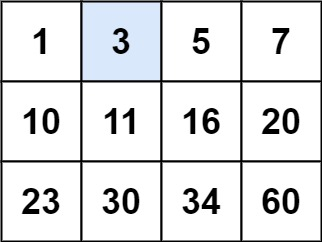
\includegraphics[width=0.2\linewidth]{images/lc0074_example1}
		\label{fig:lc0074example1}
	\end{figure}
	\item {\colorbox{CodeBackground}{\lstinline|matrix = [[1,3,5,7],[10,11,16,20],[23,30,34,60]], target = 13 --> false|}}
	\begin{figure}[H]
		\centering
		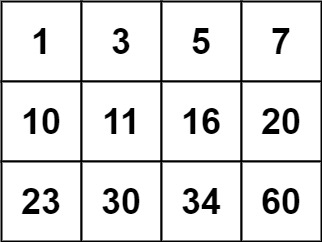
\includegraphics[width=0.2\linewidth]{images/lc0074_example2}
		\label{fig:lc0074example2}
	\end{figure}
\end{itemize}

\subsection*{Solution - One Binary Search}
\begin{lstlisting}
bool searchMatrix(std::vector<std::vector<int>>& matrix, int target) {
  int m = matrix.size();
  int n = matrix[0].size();
  int left = 0;
  int right = m * n - 1;
  while (left <= right) {
    int mid_idx = left + (right - left) / 2;
    int mid_val = matrix[mid_idx / n][mid_idx % n];
    if (target == mid_val) {
      return true;
    } else if (target < mid_val) {
      right = mid_idx - 1;
    } else {
      left = mid_idx + 1;
    }
  }
  return false;
}
\end{lstlisting}

\subsection*{Solution - Two Binary Searches}
\begin{lstlisting}
bool searchMatrix(std::vector<std::vector<int>>& matrix, int target) {
  // find the row
  int row = -1;
  int top = 0;
  int bottom = matrix.size() - 1;
  while (top <= bottom) {
    int mid = top + (bottom - top) / 2;
    if (target >= matrix[mid].front() && target <= matrix[mid].back()) {
      row = mid;
      break;
    } else if (target < matrix[mid].front()) {
      bottom = mid - 1;
    } else {
      top = mid + 1;
    }
  }
  if (row == -1) { return false; }
  // find the column
  int left = 0;
  int right = matrix[row].size() - 1;
  while (left <= right) {
    int mid = left + (right - left) / 2;
    if (target == matrix[row][mid]) {
      return true;
    } else if (target < matrix[row][mid]) {
      right = mid - 1;
    } else {
      left = mid + 1;
    }
  }
  return false;
}
\end{lstlisting}

\section{LC 0034 - Find First and Last Position of Element in Sorted Array}
Given an array of integers {\colorbox{CodeBackground}{\lstinline|nums|}} sorted in \ul{non-decreasing order}, return the starting and ending position of a given {\colorbox{CodeBackground}{\lstinline|target|}} value. If {\colorbox{CodeBackground}{\lstinline|target|}} is not found in the array, return {\colorbox{CodeBackground}{\lstinline|[-1, -1]|}}.\\

Examples:
\begin{itemize}
	\item {\colorbox{CodeBackground}{\lstinline|nums = [5,7,7,8,8,10], target = 8 --> [3,4]|}}
	\item {\colorbox{CodeBackground}{\lstinline|nums = [5,7,7,8,8,10], target = 6 --> [-1,-1]|}}
	\item {\colorbox{CodeBackground}{\lstinline|nums = [], target = 0 --> [-1,-1]|}}
\end{itemize}

\subsection*{Solution - Binary Search}
\begin{lstlisting}
std::vector<int> searchRange(std::vector<int>& nums, int target) {
  if (nums.empty()) { return {-1, -1}; }
  int first = findFirst(nums, target);
  int last = findLast(nums, target);
  return {first, last};
}

int findFirst(const std::vector<int>& nums, int target) {
  int idx = -1;
  int left = 0;
  int right = nums.size() - 1;
  while (left <= right) {
    int mid = left + (right - left) / 2;
    if (target == nums[mid]) {
      idx = mid;
      right = mid - 1;
    } else if (target < nums[mid]) {
      right = mid - 1;
    } else {
      left = mid + 1;
    }
  }
  return idx;
}

int findLast(const std::vector<int>& nums, int target) {
  int idx = -1;
  int left = 0;
  int right = nums.size() - 1;
  while (left <= right) {
    int mid = left + (right - left) / 2;
    if (target == nums[mid]) {
      idx = mid;
      left = mid + 1;
    } else if (target < nums[mid]) {
      right = mid - 1;
    } else {
      left = mid + 1;
    }
  }
  return idx;
}
\end{lstlisting}

\section{LC 0658 - Find K Closest Elements In Sorted Array}\label{lc0658}
Given a \ul{non-empty} \ul{sorted} integer array {\colorbox{CodeBackground}{\lstinline|arr|}}, two integers {\colorbox{CodeBackground}{\lstinline|k|}} ({\colorbox{CodeBackground}{\lstinline|k >= 1|}}) and {\colorbox{CodeBackground}{\lstinline|x|}}, return the {\colorbox{CodeBackground}{\lstinline|k|}} closest integers to {\colorbox{CodeBackground}{\lstinline|x|}} in the array. \\

The result should also be \ul{sorted in ascending order}.\\

An integer {\colorbox{CodeBackground}{\lstinline|a|}} is closer to {\colorbox{CodeBackground}{\lstinline|x|}} than an integer {\colorbox{CodeBackground}{\lstinline|b|}} if:
\begin{itemize}
\item {\colorbox{CodeBackground}{\lstinline|\|a - x\| < \|b - x\||}}, or
\item {\colorbox{CodeBackground}{\lstinline|\|a - x\| == \|b - x\||}} and {\colorbox{CodeBackground}{\lstinline|a < b|}}
\end{itemize}

Examples:
\begin{itemize}
\item {\colorbox{CodeBackground}{\lstinline|arr = [1,2,3,4,5], k = 4, x = 3 --> [1,2,3,4]|}}
\item {\colorbox{CodeBackground}{\lstinline|arr = [1,2,3,4,5], k = 4, x = -1 --> [1,2,3,4]|}}
\end{itemize}

\subsection*{Solution 1 - Binary Search}
\begin{lstlisting}
std::vector<int> findClosestElements(std::vector<int>& arr, int k, int x) {
  int left = 0;
  int right = arr.size() - k;
  while (left < right) {
    int mid = left + (right - left) / 2;
    if (x - arr[mid] > arr[mid + k] - x) {
      left = mid + 1;
    } else {
      right = mid;
    }
  }
  return std::vector<int>(arr.begin() + left, arr.begin() + left + k);
}
\end{lstlisting}

\subsection*{Solution 2 - Binary Search + Expand From Center}
\begin{lstlisting}
std::vector<int> findClosestElements(std::vector<int>& arr, int k, int x) {
  // binary search to find the closest element
  int left = 0;
  int right = arr.size() - 1;
  while (left < right) {
    int mid = left + (right - left) / 2;
    if (x <= arr[mid]) {
      right = mid;
    } else {
      left = mid + 1;
    }
  }
  // expand outwards to find the k closest elements
  int low = left - 1;
  int high = left;
  while (k--) {
    if (low < 0 || (high < arr.size() && std::abs(arr[high] - x) < std::abs(arr[low] - x))) {
      ++high;
    } else {
      --low;
    }
  }
  return std::vector<int>(arr.begin() + low + 1, arr.begin() + high);
}
\end{lstlisting}

\section{LC 0162 - Find Peak Element in Sorted Array}
A \ul{peak element} is an element that is \ul{strictly greater} than its neighbors.\\

Given a \ul{non-empty} {\colorbox{CodeBackground}{\lstinline|0|}}-indexed integer array {\colorbox{CodeBackground}{\lstinline|nums|}}, find a peak element, and return its index. If the array contains multiple peaks, return the index to any of the peaks.\\

Note that:
\begin{itemize}
	\item You may imagine that {\colorbox{CodeBackground}{\lstinline|nums[-1] = nums[n] = -inf|}}.
	\item {\colorbox{CodeBackground}{\lstinline|nums[i] != nums[i + 1]|}} for all valid {\colorbox{CodeBackground}{\lstinline|i|}}.
\end{itemize}

Examples:
\begin{itemize}
	\item {\colorbox{CodeBackground}{\lstinline|nums = [1,2,3,1] --> 2|}}
	\item {\colorbox{CodeBackground}{\lstinline|nums = [1,2,1,3,5,6,4] --> 5|}}
\end{itemize}

\subsection*{Solution - Binary Search}
\begin{lstlisting}
int findPeakElement(std::vector<int>& nums) {
  int left = 0;
  int right = nums.size() - 1;
  while (left < right) {
    int mid = left + (right - left) / 2;
    if (nums[mid] > nums[mid + 1]) {
      // if the mid element is greater than the next one, then a peak must be on the left
      // side, including mid.
      right = mid;
    } else {
      // if the mid element is less than or equal to the next one, then a peak must be on the
      // right side, excluding mid.
      left = mid + 1;
    }
  }
  return left;
}
\end{lstlisting}

\section{LC 0153 - Find Minimum in Rotated Sorted Array}\label{lc0153}
Suppose an array of length {\colorbox{CodeBackground}{\lstinline|n|}} ({\colorbox{CodeBackground}{\lstinline|n >= 1|}}) sorted in \ul{ascending order} is rotated to the right between {\colorbox{CodeBackground}{\lstinline|1|}} and {\colorbox{CodeBackground}{\lstinline|n|}} times. \\

For example, the array {\colorbox{CodeBackground}{\lstinline|nums = [0,1,2,4,5,6,7]|}} might become:
\begin{itemize}
	\item {\colorbox{CodeBackground}{\lstinline|[4,5,6,7,0,1,2]|}} if it was rotated {\colorbox{CodeBackground}{\lstinline|4|}} times.
	\item {\colorbox{CodeBackground}{\lstinline|[0,1,2,4,5,6,7]|}} if it was rotated {\colorbox{CodeBackground}{\lstinline|7|}} times.
\end{itemize}

Given a \ul{non-empty} \ul{rotated} \ul{sorted} integer array {\colorbox{CodeBackground}{\lstinline|nums|}} of \ul{distinct values}, return the minimum element of this array. \\

Examples:
\begin{itemize}
	\item {\colorbox{CodeBackground}{\lstinline|nums = [3,4,5,1,2] --> 1|}}
	\item {\colorbox{CodeBackground}{\lstinline|nums = [4,5,6,7,0,1,2] --> 0|}}
	\item {\colorbox{CodeBackground}{\lstinline|nums = [11,13,15,17] --> 11|}}
\end{itemize}

\subsection*{Solution 1 - Binary Search}
\begin{lstlisting}
int findMin(std::vector<int>& nums) {
  int left = 0;
  int right = nums.size() - 1;
  while (left < right) {
    int mid = left + (right - left) / 2;
    if (nums[mid] <= nums[right]) {  // inflection point is on the left half
      right = mid;
    } else {  // infection point is on the right half
      left = mid + 1;
    }
  }
  return nums[left];
}
\end{lstlisting}

\subsection*{Solution 2 - Binary Search}
\begin{lstlisting}
int findMin(std::vector<int>& nums) {
  // edge case 1
  if (nums.size() == 1) { return nums[0]; }
  int left = 0;
  int right = nums.size() - 1;
  // edge case 2: if the array is not rotated (or rotated a complete cycle)
  if (nums[left] < nums[right]) { return nums[left]; }
  // binary search to find the inflection point
  while (left <= right) {
    int mid = left + (right - left) / 2;
    // if mid element is greater than its next element, then mid + 1 element is the minimum
    if (nums[mid] > nums[mid + 1]) { return nums[mid + 1]; }
    // if mid element is less than its previous element, then mid element is the minimum
    if (nums[mid - 1] > nums[mid]) { return nums[mid]; }
    if (nums[mid] <= nums[left]) {  // inflection point is on the left half
      right = mid - 1;
    } else {  // infection point is on the right half
      left = mid + 1;
    }
  }
  return -1;
}
\end{lstlisting}

\subsection*{Related - Rotated Sequence}
\begin{itemize}
\item \hyperref[lc0153]{LC 0153 - Find Minimum in Rotated Sorted Array}
\item \hyperref[lc0033]{LC 0033 - Search in Rotated Sorted Array}
\end{itemize}

\section{LC 0033 - Search in Rotated Sorted Array}\label{lc0033}
There is a \ul{non-empty} integer array {\colorbox{CodeBackground}{\lstinline|nums|}} with \ul{distinct values} sorted in \ul{ascending order}. Prior to being passed to your function, {\colorbox{CodeBackground}{\lstinline|nums|}} is possibly rotated to the left by {\colorbox{CodeBackground}{\lstinline|k|}} ({\colorbox{CodeBackground}{\lstinline|1 <= k < nums.size()|}}) elements, such that the resulting array is {\colorbox{CodeBackground}{\lstinline|[nums[k], ..., nums[n-1], nums[0], ..., nums[k-1]]|}}. For example, {\colorbox{CodeBackground}{\lstinline|[0,1,2,4,5,6,7]|}} might be rotated by {\colorbox{CodeBackground}{\lstinline|3|}} elements and become {\colorbox{CodeBackground}{\lstinline|[4,5,6,7,0,1,2]|}}.\\

Given the rotated {\colorbox{CodeBackground}{\lstinline|nums|}} and an integer {\colorbox{CodeBackground}{\lstinline|target|}}, return the index of {\colorbox{CodeBackground}{\lstinline|target|}} if it is in the rotated {\colorbox{CodeBackground}{\lstinline|nums|}}, or {\colorbox{CodeBackground}{\lstinline|-1|}} if it is not.\\

Examples:
\begin{itemize}
	\item {\colorbox{CodeBackground}{\lstinline|nums = [4,5,6,7,0,1,2], target = 0 --> 4|}}
	\item {\colorbox{CodeBackground}{\lstinline|nums = [4,5,6,7,0,1,2], target = 3 --> -1|}}
	\item {\colorbox{CodeBackground}{\lstinline|nums = [1], target = 0 --> -1|}}
\end{itemize}

\subsection*{Solution 1 - Binary Search}
\begin{lstlisting}
int search(std::vector<int>& nums, int target) {
  int left = 0;
  int right = nums.size() - 1;
  while (left <= right) {
    int mid = left + (right - left) / 2;
    if (nums[mid] == target) { return mid; }
    if (nums[left] <= nums[mid]) {                       // if left half is sorted
      if (target >= nums[left] && target < nums[mid]) {  // if target is in the left half
        right = mid - 1;
      } else {
        left = mid + 1;  // if target is in the right half
      }
    } else {                                              // otherwise right half is sorted
      if (target > nums[mid] && target <= nums[right]) {  // if target is in the right half
        left = mid + 1;
      } else {
        right = mid - 1;  // if target is in the left half
      }
    }
  }
  return -1;
}
\end{lstlisting}

\subsection*{Solution 2 - Binary Search}
\begin{lstlisting}
int search(std::vector<int>& nums, int target) {
  int n = nums.size();
  // find the the smallest element, which is also the infelction point
  int left = 0;
  int right = n - 1;
  while (left < right) {
    int mid = left + (right - left) / 2;
    if (nums[mid] <= nums[right]) {
      right = mid;
    } else {
      left = mid + 1;
    }
  }
  int rotation = left;
  // binary search for the target
  left = 0;
  right = n - 1;
  while (left <= right) {
    int mid = left + (right - left) / 2;
    int real_mid = (mid + rotation) % n;
    if (target == nums[real_mid]) {
      return real_mid;
    } else if (target < nums[real_mid]) {
      right = mid - 1;
    } else {
      left = mid + 1;
    }
  }
  return -1;
}
\end{lstlisting}

\subsection*{Related - Rotated Sequence}
\begin{itemize}
\item \hyperref[lc0153]{LC 0153 - Find Minimum in Rotated Sorted Array}
\item \hyperref[lc0033]{LC 0033 - Search in Rotated Sorted Array}
\end{itemize}

\section{LC 0004 - Median of Two Sorted Arrays}
Given two sorted integer arrays {\colorbox{CodeBackground}{\lstinline|nums1|}} and {\colorbox{CodeBackground}{\lstinline|nums2|}} of size {\colorbox{CodeBackground}{\lstinline|m|}} and {\colorbox{CodeBackground}{\lstinline|n|}} respectively, return the \ul{median} of the two sorted arrays.\\

Examples:
\begin{itemize}
	\item {\colorbox{CodeBackground}{\lstinline|nums1 = [1,3], nums2 = [2] --> 2.00000|}}
	\item {\colorbox{CodeBackground}{\lstinline|nums1 = [1,2], nums2 = [3,4] --> 2.50000|}}
\end{itemize}

\subsection*{Solution - Binary Search}
\begin{lstlisting}
double findMedianSortedArrays(std::vector<int>& nums1, std::vector<int>& nums2) {
  // make sure nums1 is the smaller array
  if (nums1.size() > nums2.size()) { return findMedianSortedArrays(nums2, nums1); }
  int m = nums1.size();
  int n = nums2.size();
  int left = 0;
  int right = m;
  while (left <= right) {
    int partition_x = (left + right) / 2;
    int partition_y = (m + n + 1) / 2 - partition_x;
    // if partition_x is 0 it means nothing is there on left side
    int max_left_x = (partition_x == 0) ? INT_MIN : nums1[partition_x - 1];
    // if partition_x is the length of input then there is nothing on right side
    int min_right_x = (partition_x == m) ? INT_MAX : nums1[partition_x];
    // if partition_y is 0 it means nothing is there on left side
    int max_left_y = (partition_y == 0) ? INT_MIN : nums2[partition_y - 1];
    // if partition_y is the length of input then there is nothing on right side
    int min_right_y = (partition_y == n) ? INT_MAX : nums2[partition_y];
    if (max_left_x <= min_right_y
        && max_left_y <= min_right_x) {  // we have partitioned array at correct place
      if ((m + n) % 2 == 0) {
        return (std::max(max_left_x, max_left_y) + std::min(min_right_x, min_right_y)) / 2.0;
      } else {
        return std::max(max_left_x, max_left_y);
      }
    } else if (max_left_x > min_right_y) {  // we are too far on right side for partition_x
      right = partition_x - 1;
    } else {  // we are too far on left side for partition_x
      left = partition_x + 1;
    }
  }
  // if we reach here, then the arrays are not sorted properly
  throw std::invalid_argument("Input arrays are not sorted or not the right inputs.");
}

\end{lstlisting}